\chapter{Struktura systemu}
\label{sec:components}
Aby uruchomić symulację, nie wystarczy uruchomić Gazebo z modelami, należy zadbać także o odpowiednie przekazywanie informacji pomiędzy pakietami.
Wskazane jest przetestować modele, czy zachowują się poprawnie w prostych scenariuszach testowych, tak samo, jak testować się będzie program sterujący na modelu.
Do tego potrzebne są programy wspomagające, które łączy się w różne konfiguracje, w zależności od scenariusza testowego.
Ze względu na niezależność komponentów od siebie, można je także użyć przy komunikacji z rzeczywistym robotem.

\begin{table}
	\centering
	\begin{tabular}{l r}
		Typ & Opis \\
		\hline
		\texttt{omnivelma\_msgs/Encoders} & Prędkości i pozycje kół z enkodera. \\
		\texttt{omnivelma\_msgs/Vels} & Prędkości kół. \\
		\texttt{omnivelma\_msgs/SetFriction} & Nadanie tarcia elementowi modelu. \\
		\texttt{omnivelma\_msgs/SetInertia} & Nadanie mas i momentu bezwładności obiektowi. \\
		\texttt{geometry\_msgs/Pose} & Pozycja i rotacja obiektu w przestrzeni kartezjańskiej. \\
		\texttt{geometry\_msgs/Twist} & Prędkość względna obiektu. \\
		\texttt{sensor\_msgs/LaserScan} & Jedno skanowanie LiDARa, wraz z nagłówkiem. \\
		\texttt{omnivelma\_msgs/Relative} & Odległość i kąt pomiędzy obiektami. \\
		\texttt{nav\_msgs/Odometry} & Transformacja obiektu z macierzą kowariancji. \\
		\texttt{sensor\_msgs/Imu} & Dane generowane przez czujnik inercji. \\
	\end{tabular}
	\caption{Typy i opisy wiadomości przekazywanych pomiędzy komponentami.}
	\label{tab:messages}
\end{table}

Niektóre typy wiadomości mają dopisek \texttt{Stamped}, co oznacza że zawierają także nagłówek.
Nagłówek posiada trzy pola:
\begin{itemize}
	\item Numer sekwencyjny, zwiększany przez program wysyłający po każdym pakiecie.
	\item Czas nadania pakietu, z dokładnością do nanosekund.
	\item Identyfikator ramki, według której podano dane, ramki zostały opisane dokładniej w sekcji \ref{sec:frames}.
\end{itemize}

Komponenty można podzielić na trzy typy:
\begin{itemize}
	\item Generujące pakiety danych.
	\item Przekazujące i modyfikujące pakiety danych.
	\item Zbierające pakiety danych.
\end{itemize}
Poniżej, każdy pakiet opisany jest bardziej szczegółowo, ten dokument nie ma za zadanie być programistyczną dokumentacją komponentów, dlatego 
nie zagłębia się dokładnie w argumenty, algorytmy i technologie programów.

W ostatecznym działaniu symulatora, podłączenie komponentów będzie wyglądać następująco:
\begin{figure}[H]
	\centering
	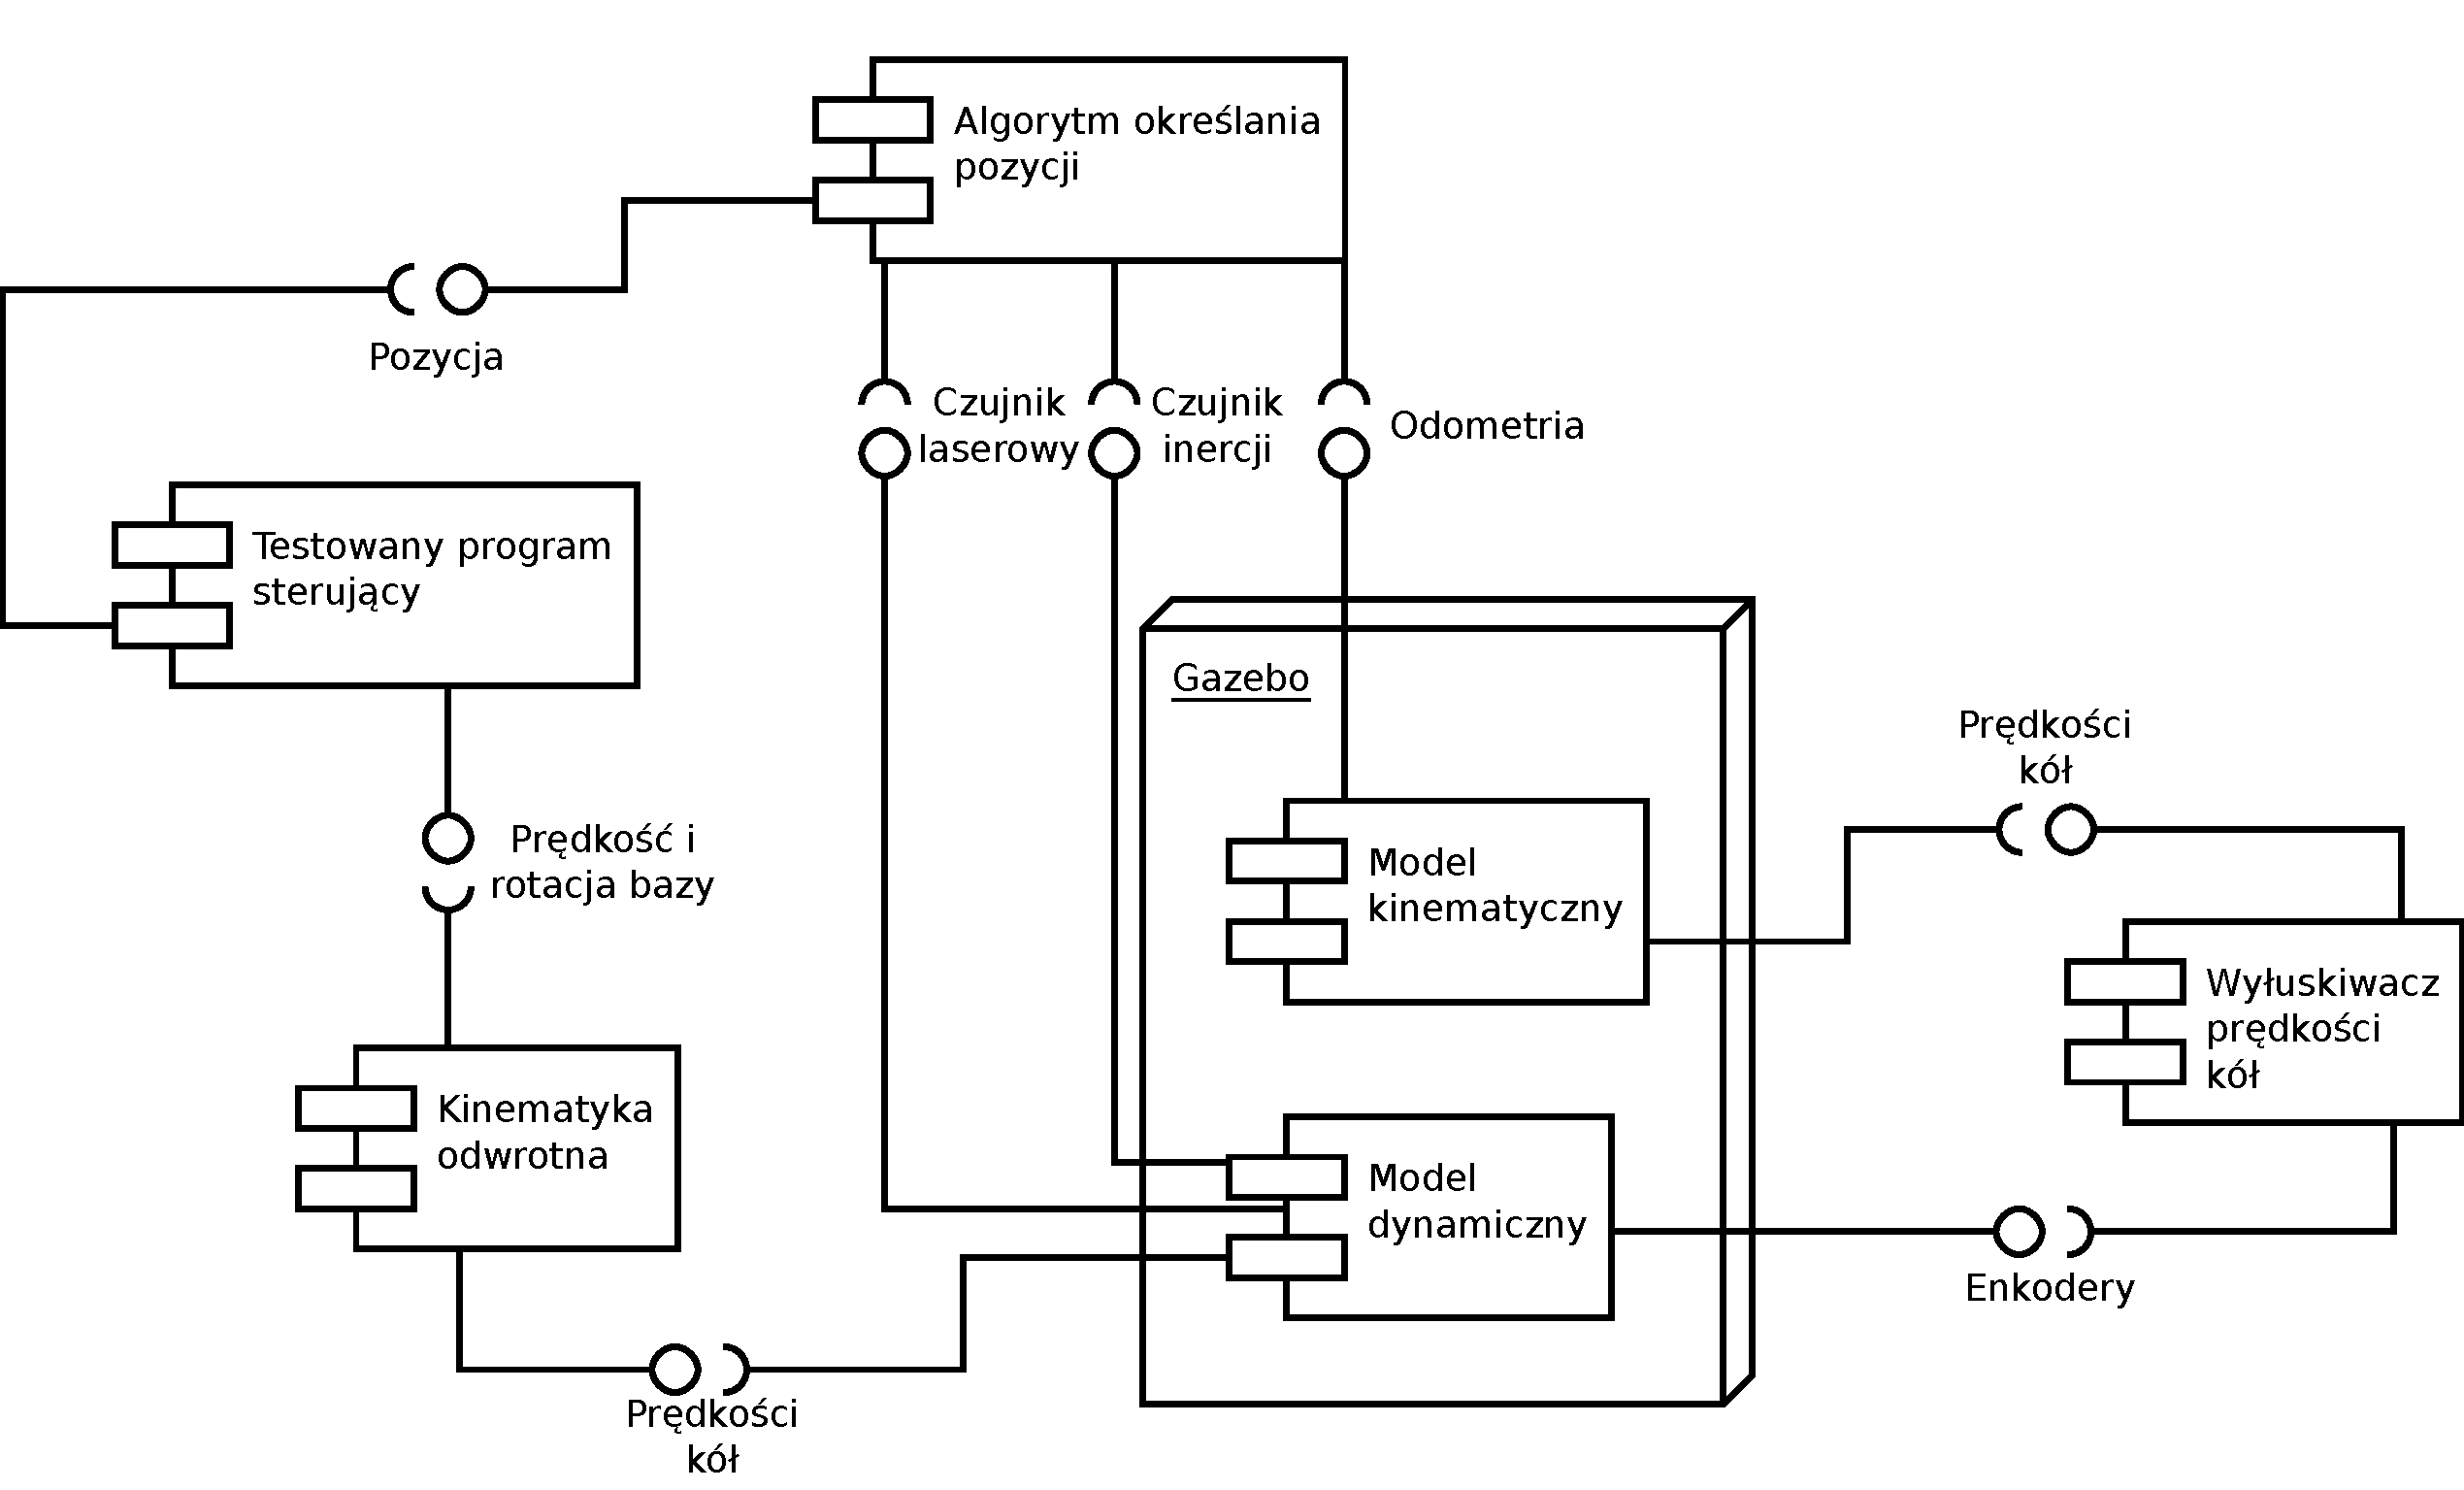
\includegraphics[width=\textwidth]{uml/final.pdf}
	\caption{Komunikacja podstawowych komponentów systemu w trakcie testowania programu sterującego.}
\end{figure} 

Ważną rolę odgrywa tutaj algorytm określania pozycji, bazujący na odometrii, czujniku inercji i danych z czujnika laserowego.
Odometria jest generowana za pomocą modelu kinematycznego, sterowanego danymi z enkoderów modelu dynamicznego.
Sam model dynamiczny sterowany jest pośrednio przez program, który generuje zadane prędkości i obrót robota.
W uproszczeniu: program sterujący wysyła sterowanie do modelu, bazując na jego pozycji, określonej z danych generowanych przez modele czujników.

W każdym miejscu przepływu danych można zebrać i zwizualizować przesyłane wartości.
Program sterujący może także korzystać z czujników laserowych w celu wykrycia przeszkody, nie tylko w celu określenia pozycji.
Bardziej zaawansowany program sterujący mógłby generować zadane prędkości kół bezpośrednio.

Komponenty modeli platform i czujnika laserowego, zostały opisane szczegółowo w poprzednich sekcjach.

\begin{description}
	\item[\texttt{omnivelma}] Model platformy dynamicznej w sekcji \ref{sec:omnivelma}.
	\item[\texttt{pseudovelma}] Model platformy kinematycznej w sekcji \ref{sec:pseudovelma}.
	\item[\texttt{monokl}] Model czujnika laserowego w sekcji \ref{sec:monokl}.
\end{description}

\section{Manualne sterowanie}
\label{sec:lalkarz}
	To zaawansowany program do manualnego generowania zadanych prędkości, lub kierunku platformy.
	Ponieważ jest niezależny od reszty systemu, może być użyty do sterowania rzeczywistym robotem.
	Pozwala także na wyświetlanie aktualnych prędkości kół, generowanych przez enkodery.
	Ma nazwę kodową \texttt{lalkarz}, ponieważ steruje platformą, tak jak aktor steruje marionetką.
	
	\subsection{Program}
		Ten komponent jest plikiem wykonywalnym, skompilowanym ze źródeł w C++.
		Wykorzystując bibliotekę graficzną SFML, generuje okno z powierzchnią do rysowania na nim za pomocą OpenGL.
		Biblioteka ta pozwala również na bezproblemowe przechwytywanie zdarzeń z klawiatury, takich jak wciśnięcie i puszczenie klawisza, a także na obsługę kontrolera go gier i myszki.
		Za pomocą gałek kontrolera, można nadawać robotowi niebinarne prędkości kół, co jest niezbędne do płynnego i bezpiecznego kontrolowania urządzeniem.
		Użyto także sterowania kursorem myszy, w razie gdyby użytkownik nie posiadał kontrolera.
		
		Aplikacja tego typu mogłaby bez większego problemu pracować z interfejsem tekstowym w terminalu, aby być bardziej przenośna i lżejsza w zasobach, 
		lecz nie mogłaby wykrywać zdarzeń puszczenia klawisza
		(bez bezpośredniego czytania z urządzenia \texttt{/dev/input/eventX}, do czego są potrzebne prawa roota). 
		Dodatkowo, interfejs graficzny pozwala na wyświetlenie dokładniejszych wskaźników i elementów wskazujących.
		
		Program uruchamiany jest z wiersza polecenia, z argumentami dotyczącymi nazw strumieni i początkowej konfiguracji urządzenia.
	
	\subsection{Komunikacja}
		Program potrafi generować dwa typy wiadomości.
		
		Pierwszą są prędkości kół \texttt{omnivelma\_msgs/Vels}, jakie w danej chwili platforma powinna przyjąć na sterowanie.
		Pozwala to na dokładne przetestowanie zachowania się modelu platformy.
		Można także wywołać takie prędkości, które nie powinny być używane przy rzeczywistym sterowaniu, gdyż wprowadzają duże nieścisłości ruchu 
		(przykładowo, obracanie przednich i tylnych kół tak, aby ich wektory prędkości się znosiły, będzie nadawać niedeterministyczny ruch, spowodowany niedoskonałościami
		pojedynczych rolek).
		
		Drugi typ wiadomości, \texttt{geometry\_msgs/Twist}, to nadana prędkość względna platformy.
		To intuicyjny sposób, w jaki użytkownik steruje platformą i w jaki sposób mógłby także sterować nią prosty program sterujący.
		Jednak ponieważ ani model platformy, ani rzeczywisty robot nie są wstanie poruszać się bez informacji, jakimi kołami z jaką prędkością obracać,
		ten typ wiadomości musi być jeszcze konwertowany przez komponent modelu kinematyki odwrotnej, opisany w sekcji \ref{sec:transmutator}.
		
		Program opcjonalnie przyjmuje także wiadomość \texttt{omnivelma\_msgs/Vels}, aby wyświetlić dane enkoderów.
		Należy zauważyć, że nie przyjmuje całego pakietu \texttt{omnivelma\_msgs/EncodersStamped}, jaki jest generowany przez model platformy,
		a jedynie mały ich wycinek, gdyż tylko te informacje jest w stanie wyświetlić i tylko takie potrzebuje.
		Dzięki temu może być użyty niezależnie od innych komponentów i programów. Jednak może być wymagane użycie dodatkowego komponentu do 
		wyłuskania tej informacji z większego pakietu,
		patrz \ref{sec:dziadzio}.
		
	\subsection{Tryby działania}
		Program posiada 11 trybów działania, w których generuje różne wiadomości w różny sposób.
		Jedne są bardziej przydatne, inne bardzo proste i służące do ogólnej prezentacji systemu.
		Globalny mnożnik wyjścia pozwala na łatwe ograniczenie generowanych danych i ustawienia dokładności. Spacja awaryjnie zeruje wszystkie wyjścia.
		\begin{enumerate}
			\item Za pomocą ośmiu klawiszy klawiatury numerycznej, można nadać platformie określone prędkości kół.
			W tym trybie, koło może albo stać w miejscu, albo obracać się z odpowiednią prędkością, w określonym kierunku. 
			Powoduje to naturalne szarpnięcia i poślizgi platformy. W trakcie braku aktywności użytkownika, platforma stoi w miejscu.
			\item Podobnie do poprzedniego trybu, lecz przy braku naciśnięcia klawisza, generuje cichą nie-liczbę, aby zachować aktualną prędkość kół modelu.
			Ta dodatkowa funkcjonalność opisana jest szerzej w sekcji \ref{sec:model_nan}.
			\item Naciśnięcie klawisza płynnie zwiększa, lub zmniejsza prędkość koła. W trakcie braku aktywności użytkownika, platforma porusza się 
			z ustawionymi prędkościami kół.
			\item Podobnie, co w poprzednim trybie, lecz pozwala na schodkowe ustawienie prędkości kół co 0,1 $\frac{rad}{s}$ (pomnożone przez dokładność).
			Dzięki temu, możliwe jest w miarę dokładne powtórzenie manualnych testów platformy.
			\item Poprzedni tryb, lecz przy ustawieniu prędkości zerowej, generuje nie-liczbę.
			\item Sterowanie prędkościami kół za pomocą gałek kontrolera.
			Większość kontrolerów posiada dwa, dwuosiowe joysticki, co daje cztery osie, zmieniające się w zakresie $\left<-1;1\right>$.
			Można za ich pomocą bezpośrednio ustawiać prędkości kół, chociaż jest to nieintuicyjne w działaniu.
			\item Lokalny kierunek jazdy platformy składa się z dwóch wektorów prędkości liniowej i wektora obrotu. 
			Za pomocą klawiatury, binarnie, można nadać platformie jeden z ośmiu kierunków poruszania się i jeden z dwóch kierunków obrotu.
			Ponownie, ta metoda sterowania powoduje skoki prędkości i poślizgi. Przypomina sterowanie pojazdami w grach komputerowych.
			Puszczenie klawiszy powoduje zatrzymanie się platformy.
			\item Podobny tryb do poprzedniego, ale naciśnięcie klawisza płynnie dodaje wartość do kierunku poruszania się i obrotu platformy.
			Brak aktywności użytkownika powoduje, że model porusza się z zadaną prędkością w zadanym kierunku i z zadanym obrotem.
			\item Połączenie dwóch poprzednich trybów, schodkowe sterowanie prędkością platformy. Pozwala na ustawienie prędkości i obrotu platformy z zadaną dokładnością.
			\item Sterowanie kierunkiem platformy za pomocą kontrolera. Trzy osie są używane, dwie do nadania prędkości, jedna do nadania obrotu.
			Jest to prawdopodobnie najczęstszy sposób kontrolowania robotów wielokierunkowych za pomocą kontrolera.
			Bardzo intuicyjny i używany także przez inne pakiety do manualnego sterowania robotami na kołach Mecanum.
			\item Sterowanie za pomocą myszki, najdokładniejsze sterowanie kierunkiem, mniej dokładne obrotem.
			Kursor myszy wskazuje końcówkę strzałki reprezentującej kierunek ruchu robota, za pomocą kółka, można dodawać, lub odejmować prędkość do obrotu wokół osi.
			Ponieważ większość myszek ma skokowe obroty kółek, wprowadza to nieznaczne poślizgi. Można także modyfikować obrót klawiaturą w płynnym trybie przyrostowym.
		\end{enumerate}
		
		\begin{figure}[H]
		\centering
		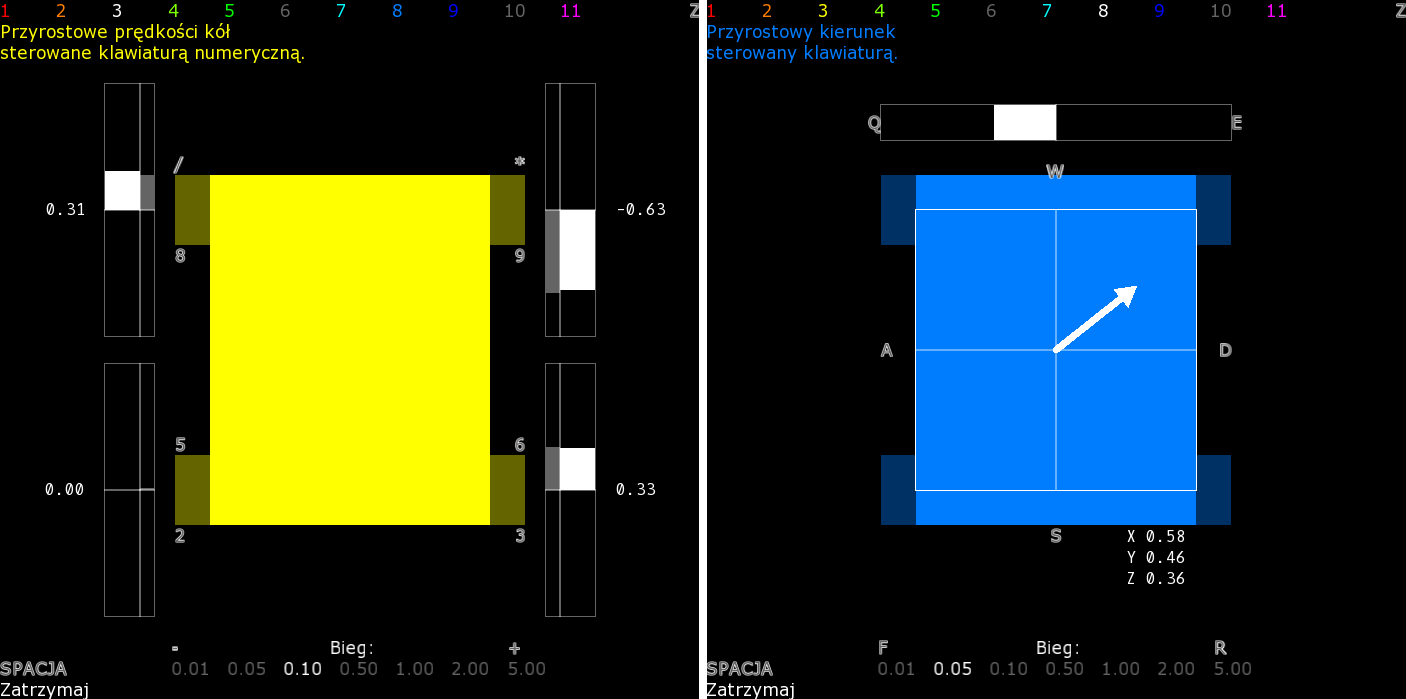
\includegraphics[width=\textwidth]{graphics/lalkarz.png}
		\caption{Zrzuty ekranu dwóch trybów działania programu.}
		\label{fig:lalkarz}
		\end{figure}
		
		Interfejs składa się z listy trybów, wyświetlanych na górze, i nazwy aktualnego trybu.
		Wyszarzone tryby nie mogą być aktywowane, w tym przypadku z powodu braku podłączenia kontrolera.
		
		Na lewym zrzucie widać zarys platformy i białe wskaźniki aktualnych prędkości kół, wraz ze współczynnikiem wypełnienia.
		Obok nich znajdują się szare wskaźniki prędkości, zwrócone przez modele enkoderów.
		Małe, szare znaki to nazwy klawiszy, używanych w tym trybie do modyfikowania prędkości.
		
		Na prawym obrazku jest tryb generowania kierunku i obrotu. Strzałka wskazuje wektor prędkości, a górny pasek obrót platformy.
		
		Na dole jest lista ,,biegów'' urządzenia, są to zwyczajne mnożniki wyjścia w celu wygodnego przestawiania dokładności z jaką platforma powinna się poruszać.
		
		Wszystkie dane są w jednostkach SI, tzn, efektywna prędkość koła będzie się równać liczbie podanej przy kole, pomnożonej przez aktualny bieg.
		Dla obrotów to są $\frac{rad}{s}$, dla prędkości to $\frac{m}{s}$.
		
\section{Generator sterowania}
	\label{sec:gramofon}
	Podstawą przeprowadzania testów modelu jest powtarzalność eksperymentów, oraz dokładność.
	Potrzeba zatem jest sposobu na automatyczne wygenerowanie strumienia wiadomości z określonymi danymi.
	
	Program \texttt{gramofon} wczytuje plik danych, w którym znajdują się rekordy, każdy opisuje:
	\begin{itemize}
		\item Prędkość liniową platformy w osi X.
		\item Prędkość liniową platformy w osi Y.
		\item Prędkość kątową platformy w osi Z.
		\item Czas $t$, przez który program ma generować wiadomość z podanymi wyżej danymi.
	\end{itemize}
	Program czyta także z argumentu okres $T$ odświeżania wiadomości.
	
	Korzystając z dwóch liczników systemowych, program generuje co $T$ sekund wiadomość typu \texttt{geometry\_msgs/Twist} z danymi aktualnie wykonywanej linii pliku.
	Ta wiadomość powtarza się regularnie.
	
	Po upływie czasu $t$, program nadaje dodatkową wiadomość z nowymi danymi, oraz przestawia dane generowane przez wywołania pierwszego licznika.
	
	Po wykorzystaniu danych, algorytm nadal generuje wiadomości z zerowymi prędkościami, aby zatrzymać model platformy i podtrzymać aktywne hamowanie kół.
	
	W ten sposób, możliwe jest proste generowanie sterowania robota, bazujące na czasie.
	Przykładowo, program może generować sterowanie:
	\begin{enumerate}
		\item Ruch przez 3,2 s, z prędkością 0,2 $\frac{m}{s}$, w kierunku (2,1).
		\item Zatrzymanie na czas 0,9 s.
		\item Obrót przez czas 10 s, z prędkością kątową 0,02 $\frac{rad}{s}$.
	\end{enumerate}
	
	Ponieważ jednak system operacyjny, na którym pracuje program i symulator, nie spełnia wymogów systemu czasu rzeczywistego, generowane wiadomości
	nie muszą być (i nie są) wysyłane dokładnie w określonych momentach. Można przeprowadzić prosty eksperyment, aby zaprezentować ten problem.
	
	\begin{figure}[H]
	\centering
	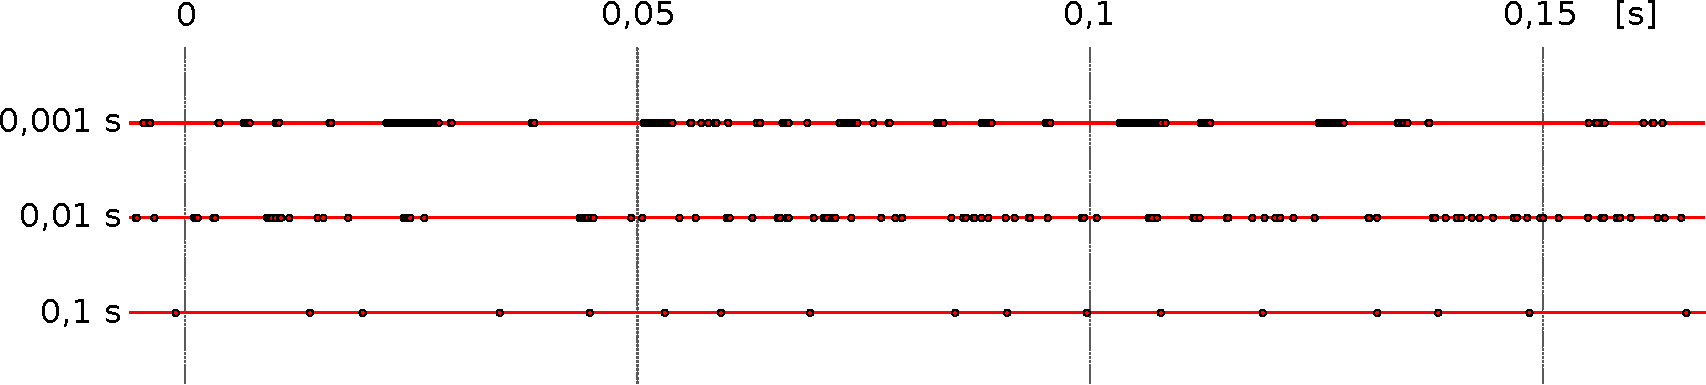
\includegraphics[width=\textwidth]{graphics/gramofon.pdf}
	\caption{Czas odbioru pakietu, wysyłanego przez program działający z jednym z trzech okresów.}
	\end{figure}
	
	Działa to tak samo, jakby każdą wiadomość wysyłać z losowym opóźnieniem.
	Gdy nadań jest za dużo (górny wykres), system zaczyna je buforować, a co za tym idzie, nadaje je w grupach o losowej wielkości.
	Pakiet po nadaniu przechodzi przez wiele procesów, każdy może nadawać losowe opóźnienie dla wiadomości.
	System operacyjny pod dużym obciążeniem przez inne procesy będzie opóźniał i buforował wiadomości o niższych częstotliwościach.
	
	Aby rozwiązać ten problem, należałoby uruchomić całe środowisko ROSa na systemie operacyjnym czasu rzeczywistego.
	Jedynym takim systemem, eksperymentalnie wspieranym przez twórców ROSa, jest OpenEmbedded.
	Jednakże budowa i uruchomienie tego systemu jest bardzo złożone.
		
\section{Wyłuskanie struktury wiadomości}
	\label{sec:dziadzio}
	Każda wiadomość przekazywana pomiędzy komponentami jest zwykle zagnieżdżoną strukturą.
	Na przykład pakiet typu \texttt{geometry\_msgs/Twist} składa się z dwóch podstruktur wektorów trójwymiarowych.
	Jeden odpowiada za prędkość, a drugi za rotację.
	
	Czasami może zdarzyć się, że jakiś komponent potrzebuje jedynie wewnętrznej podstruktury pakietu.
	Nie powinno mu się zatem przekazywać całej struktury wiadomości, gdyż to powodowałoby niepotrzebne opóźnienia, oraz nie pozwoliłoby zachować niezależności 
	komponentu od innych.
	
	Takie zjawisko występuje przy przekazywaniu informacji o pozycji i prędkości kół, generowanej przez model czujnika enkoderów, do programu
	manualnego sterowania, opisanego w \ref{sec:lalkarz}.
	
	ROS nie pozwala na automatyczne odbieranie tylko części pakietu, dlatego powstał program o nazwie kodowej \texttt{dziadzio}, niczym dziadek do orzechów.
	Przyjmuje wiadomości typu \texttt{omnivelma\_msgs/EncodersStamped} i zwraca wiadomości typu \texttt{omnivelma\_msgs/Vels}, który to typ 
	jest zawarty wewnątrz przyjmowanej struktury. Pozwala to na połączenie modelu czujnika enkoderów z wyświetlaczem prędkości kół w programie do manualnego sterowania.

\section{Podłoga o zmiennym współczynniku tarcia}
	\label{sec:flooria}
	Symulacja nie składa się jedynie z robota i czujnika, ale także z podłoża, na którym musi się poruszać.
	Ponieważ podłoże również wpływa na symulację, powinien istnieć sposób na ustawienie jego współczynnika tarcia.
	Robi się to wewnętrznie w identyczny sposób, jak w przypadku kół platformy, co zostało opisane w sekcji \ref{sec:friction}.
	
	W tym przypadku jednak powinno się ustawić identyczne wektory tarć $F_1$ i $F_2$, aby podłoże symulowało równe tarcie we wszystkich kierunkach.
	Tak samo, jak w przypadku modelu platformy dynamicznej, program nadający podłożu odpowiednie wektory tarcia przyjmuje asynchroniczne wywołanie 
	typu \texttt{omnivelma\_msgs/SetFriction}, zawierające dwie wartości zmiennoprzecinkowe.
	
	Nazwa kodowa tego programu sterującego to \texttt{flooria}, od angielskiej nazwy na podłogę.
	Program jest uruchamiany jako biblioteka symulatora Gazebo.
	
\section{Algorytm usuwania szumu z danych modelu czujnika inercji}
	\label{sec:odszumiacz}
	Jak wcześniej wspomniano, różniczkowanie prędkości w maszynie symulacji fizyki generuje duże błędy.
	
	Ten program uśrednia dane w prosty sposób, licząc średnią z określonej ilości poprzednich pomiarów.
	Odczytuje nazwę nadajnika i odbiornika wiadomości typu \texttt{sensor\_msgs/Imu}, oraz wielkość bufora,
	
	Taki algorytm nie sprawdza się jednak, gdy dane są generowane naprzemiennie.
	Na przykład, jeśli w jednej klatce symulacji maszyna do symulacji fizyki obliczy prawidłową wartość, a w drugiej zwróci zerową,
	to ten algorytm uśredni te wyniki i zwróci wartość pośrodku.
	
	Jednak stworzenie tego komponentu pozwoliło sprawdzić, czy model czujnika inercji reaguje na ruch platformy z określonymi przyspieszeniami.
	Pozwolił także na odkrycie innych cech generatora.
	Używany jest w przeprowadzeniu testów w sekcji \ref{sec:test_imu}. Nazwa kodowa to \texttt{odszumiacz}.
	
\section{Obserwator symulacji}
	\label{sec:ocznica}
	Kolejny program uruchamiany w symulatorze Gazebo, oblicza i zwraca ciąg danych, reprezentujący 
	odległość i kąt pomiędzy platformą dynamiczną i kinematyczną, pakiet \texttt{omnivelma\_msgs/Relative}.
	Te dane pozwalają sprawdzić, na ile symulacja fizyczna opóźnia się względem matematycznego modelu.
	
	Ten program nie może być zaimplementowany jako zewnętrzny komponent, gdyż wiadomości zawierające pozycje platform będą przychodzić asynchronicznie.
	Nie da się w takim przypadku obliczyć dokładnych odległości pomiędzy platformami w danej chwili. 
	Wprowadzałoby to także spore opóźnienie, gdyż program musiałby czekać na odbiór obu pakietów, dodatkowo zachowując pewność że oba pochodzą z tej samej klatki symulacji.
	
	Nazwa kodowa tego programu to \texttt{ocznica}.
	
\section{Model kinematyki odwrotnej}
	\label{sec:transmutator}
	Jest to model kinematyki odwrotnej, alternatywa do modelu kinematycznego, opisanego w sekcji \ref{sec:pseudovelma}, jednak działającego bez symulatora i bez możliwości 
	całkowania prędkości (i generowania danych o aktualnej pozycji).
	Ten komponent przyjmuje zadaną prędkość, kierunek i obrót platformy, a zwraca prędkości kół, które powinny być nadane platformie, aby wywołać taki ruch.
	
	\begin{equation}
	\begin{bmatrix}
	\omega_1 \\
	\omega_2 \\
	\omega_3 \\
	\omega_4 \\
	\end{bmatrix}
	=
	\frac{1}{r}
	\begin{bmatrix}
	1 & -1 & \frac{a+b}{2} \\
	1 & 1 & -\frac{a+b}{2} \\
	1 & -1 & -\frac{a+b}{2} \\
	1 & 1 & \frac{a+b}{2} \\
	\end{bmatrix}
	\begin{bmatrix}
	v_y \\
	v_x \\
	\omega_z \\
	\end{bmatrix}
	\end{equation}
	
	Stałe, użyte we wzorze zdefiniowane są w tabeli \ref{tab:dims}, a numerowanie kół na rysunku \ref{fig:base_dims}.
	Ten wzór, podobnie jak poprzedni, pojawia się w wielu pracach, na przykład \cite{wheels}, dokładny wygląd macierzy zależy od numerowania kół i interpretacji kierunków osi.
	
	Dodatkowo, program pozwala na obrót wektora prędkości o kąt prosty, lub półpełny. 
	Jest to spowodowane tym, że różne komponenty i różne modele przyjmują różną pozycję wyjściową robota.
	Czasami przód modelu skierowany jest w dodatnią stronę osi X, a czasami Y. W związku z tym, ta funkcjonalność jest w stanie przekonwertować dane wejściowe dla innego robota.
	
	Nazwa kodowa to \texttt{transmutator}, wykonuje transmutację jednego typu prędkości w inny.
	
\section{Mapa z symulacją}
	Symulator Gazebo przy uruchomieniu ładuje plik zawierający referencje robotów i ich początkowe pozycje, używane w symulacji.
	Ten pakiet nie jest programem wykonywalnym, lecz prezentuje informacje dla symulatora o scenie symulacji.
	
	Plik typu \texttt{world} jest plikiem SDF, podobnym do tych, które służą do określenia wewnętrznej budowy robotów.
	Posiada listę elementów \texttt{import} ze ścieżkami modeli, a także nazwy programów działających bez modelu, jak obserwator symulacji, opisany w sekcji \ref{sec:ocznica}.

	W tym pliku zawierają się także ustawienia symulacji, jak przyspieszenie grawitacyjne, typ maszyny symulacyjnej fizyki ze współczynnikami, czy ustawienia wirtualnej atmosfery.
	
	Nazwa komponentu \texttt{velmaverse} jest zlepkiem słów ,,universe'' i nazwy robota manipulacyjnego.
	
\section{Rozdzielacz pakietów}
	Jeśli dwóm komponentom nadać te same nazwy interfejsów, to ROS będzie przekazywał pomiędzy nimi informacje.
	To jednak nie zawsze jest możliwe, aby mieć całkowitą kontrolę nad nazwami interfejsów wszystkich komponentów.
	Dlatego też, potrzeby jest program do przekazywania i ewentualnego rozdzielania pakietów dla różnych odbiorników.
	
	Ten program wykonywalny pobiera i generuje wiadomości typu \texttt{omnivelma\_msgs/Vels}, zawierające prędkości kół.
	Pozwala to na sterowanie kilkoma robotami o identycznym interfejsie ze wspólnego źródła.
	W szczególności przydaje się to przy rozdzielaniu wartości prędkości kół dla modelu platformy dynamicznej i kinematycznej.
	
	Nazwa kodowa \texttt{widelnica} jest referencją do widelca którego końcówka rozdziela się na kilka części, a także do angielskiej nazwy ,,fork'', używanej w podobnych 
	przypadkach rozdzielania informacji.
	
\section{Prosty program sterujący}
	Jest to uproszczona wersja programu, który docelowo ma być tworzony na podstawie budowanego systemu modeli.
	Pozwala on sprawdzić, jak dla prostych zasad model będzie się zachowywał.
	
	Program periodycznie wysyła wiadomość typu \texttt{geometry\_msgs/Twist} o kierunku równoległym do osi współrzędnych.
	W zależności od danych z czujników laserowych, program zmienia swój stan i obraca kierunek obrotu o 90\textdegree.
	Ten sterownik dla uproszczenia nie generuje poleceń obrotu kątowego, model powinien być zawsze zwrócony w tę samą stronę.
	
	Działanie programu oparte jest na zachowaniu akcja-reakcja.
	Dane z czujników laserowych dzielone są, w zależności od kąta pomiaru, na cztery ćwiartki lokalnego układu współrzędnych.
	Rozpatrywane są tylko te ćwiartki, w których kierunku porusza się platforma.
	Jeśli pomiar wypadnie wystarczająco blisko platformy, kierunek jest obracany w odwrotnym do tej ćwiartki kierunku.
	
	Na przykład, jeśli platforma porusza się w prawo i wykryje obiekt w trzeciej ćwiartce (czyli po prawej stronie względem aktualnego kierunku poruszania się),
	to zacznie poruszać się prosto, aby uniknąć przeszkody.
	
	Taki program gwarantuje omijanie przeszkód, aby platforma nie zderzyła się z jakimś obiektem.
	
	Nazwa kodowa \texttt{pantofelek} pochodzi z tego, że zachowuje się jak taki pierwotniak.
	
\section{Struktury pakietów wiadomości}
	Ten komponent nie jest plikiem wykonywalnym, a definicjami struktur danych, używanych przez wiadomości ROSa w projekcie, jeśli 
	standard nie obejmuje potrzebnego typu wiadomości.
	Nazwa kodowa i jednocześnie przedrostek wszystkich zawartych typów to \texttt{omnivelma\_msgs}.

\section{Zewnętrzne pakiety}
	Istnieje kilka tysięcy różnych pakietów i programów, tworzonych przez społeczność ROSa.
	
	\subsection{Rysownik wykresów}
		Pakiet \texttt{rqt-multiplot} jest wtyczką do większego programu \texttt{rqt}.
		Pozwala na generowanie dwuwymiarowych wykresów, bazując na dwóch dowolnych wartościach z odbieranych pakietów, lub czasie.
		Można porównać różne wykresy na jednym układzie.
		
		W szczególności przy ustawieniach pozycji Y względem X, pobranych z pakietu pozycji, nadawanego przez obie platformy, pozwala narysować trajektorię ruchu platform.
	\subsection{Wizualizer pomiarów}
		Oryginalnie napisany dla robota o tej samej nazwie, \texttt{rviz} prezentuje trójwymiarową przestrzeń, na której można wyświetlać 
		dane odebrane z pakietów.
		
		Pozwala to na przykład umieścić znacznik platformy i chmury punktów odebranych z czujników laserowych.
		Jest lżejszy na zasobach w działaniu niż Gazebo i pokazuje tylko informacje z odebranych danych, a nie całe środowisko symulacji.
		
	\subsection{Zbieranie danych}
		Każdy \texttt{topic} może zostać zapisany do pliku, a następnie odtworzony w ten sam sposób.
		Wbudowane w ROSa narzędzie \texttt{rosbag} pozwala ,,nagrać'' i odtworzyć dane dokładnie w taki sam sposób, w jaki zostały odebrane.
		Zapisuje to w formie pliku binarnego, wraz z dokładnymi parametrami działania nadajnika wiadomości.
		Możliwe jest również wydrukowanie danych do pliku tekstowego, aby mógł być wykorzystany przez inne programy jak Gnuplot, Calc (Exel), czy Matlab.
		
	
	
	
	
	

